%%% SVN stuff
\svnidlong
{$HeadURL: https://svn.riouxsvn.com/kneadlatxinputs/ExampleArtifactFolders/6b-STS/STS_Chapter_01.tex $}
{$LastChangedDate: 2024-03-14 00:31:03 -0400 (Thu, 14 Mar 2024) $}
{$LastChangedRevision: 94 $}
{$LastChangedBy: KneadProject $}
\svnid{$Id: STS_Chapter_01.tex 94 2024-03-14 04:31:03Z KneadProject $}

\chapter{Scope}
\label{chap:Scope}
% \DIDINFO{ALL-1.0 :: }


If applicable, each section has a summary of data item description (DID) information shown in this font.
These are displayed in small capital font and are not part of the formal document.
Display of these DID information notes can be turned off for formal releases, but are displayed here for reference.


This document provides the System Test Specification (\STS) for the \ThisSystem. 
The system will be referred to as the \ThisSys.

\section{Identification}
\label{sec:Identification}
% \DIDINFO{ALL-1.1 :: The \ThisSystem is an RP2040 based microcontroller board.}
This paragraph shall contain a full identification of the system to which this document applies, including, as applicable, 
identification number(s), title(s), abbreviation(s), version number(s), and release number(s).

The \ThisSystem described in this document shall be known as \ThisSys version 1.
However, the \STS described herein shall be applicable to pre-releases such as Beta-releases for a phased release as listed for each requirement.

\section{System Overview}
\label{sec:SystemOverview}
% \DIDINFO{ALL-1.2 :: This paragraph shall briefly state the purpose of the system to which this document applies. 
It shall describe the general nature of the system; summarize the history of system development, operation, 
and maintenance; identify the project sponsor, acquirer, user, developer, and support agencies; 
identify current and planned operating sites; and list other relevant documents. }

The \ThisSystem will be able to measure moisture levels and control irrigation in raised garden beds. 
\ThisSys is being developed by Zachary Steinberg and sponsored by University of Maryland Graduate Engineering. 
The operator and maintaner of \ThisSys will also be Zachary Steinberg. The \ThisSys will be operated outside along raised garden beds. 
\ThisSys is designed to be used by home gardeners. It is not intended for industry. \ThisSys will be controlled by a Raspberry Pi Pico W microcontroller board.

Figure~\ref{fig:SystemOverview} shows the development kit used for the \ThisSys system. 
\begin{figure}[htbp]
	\centering
		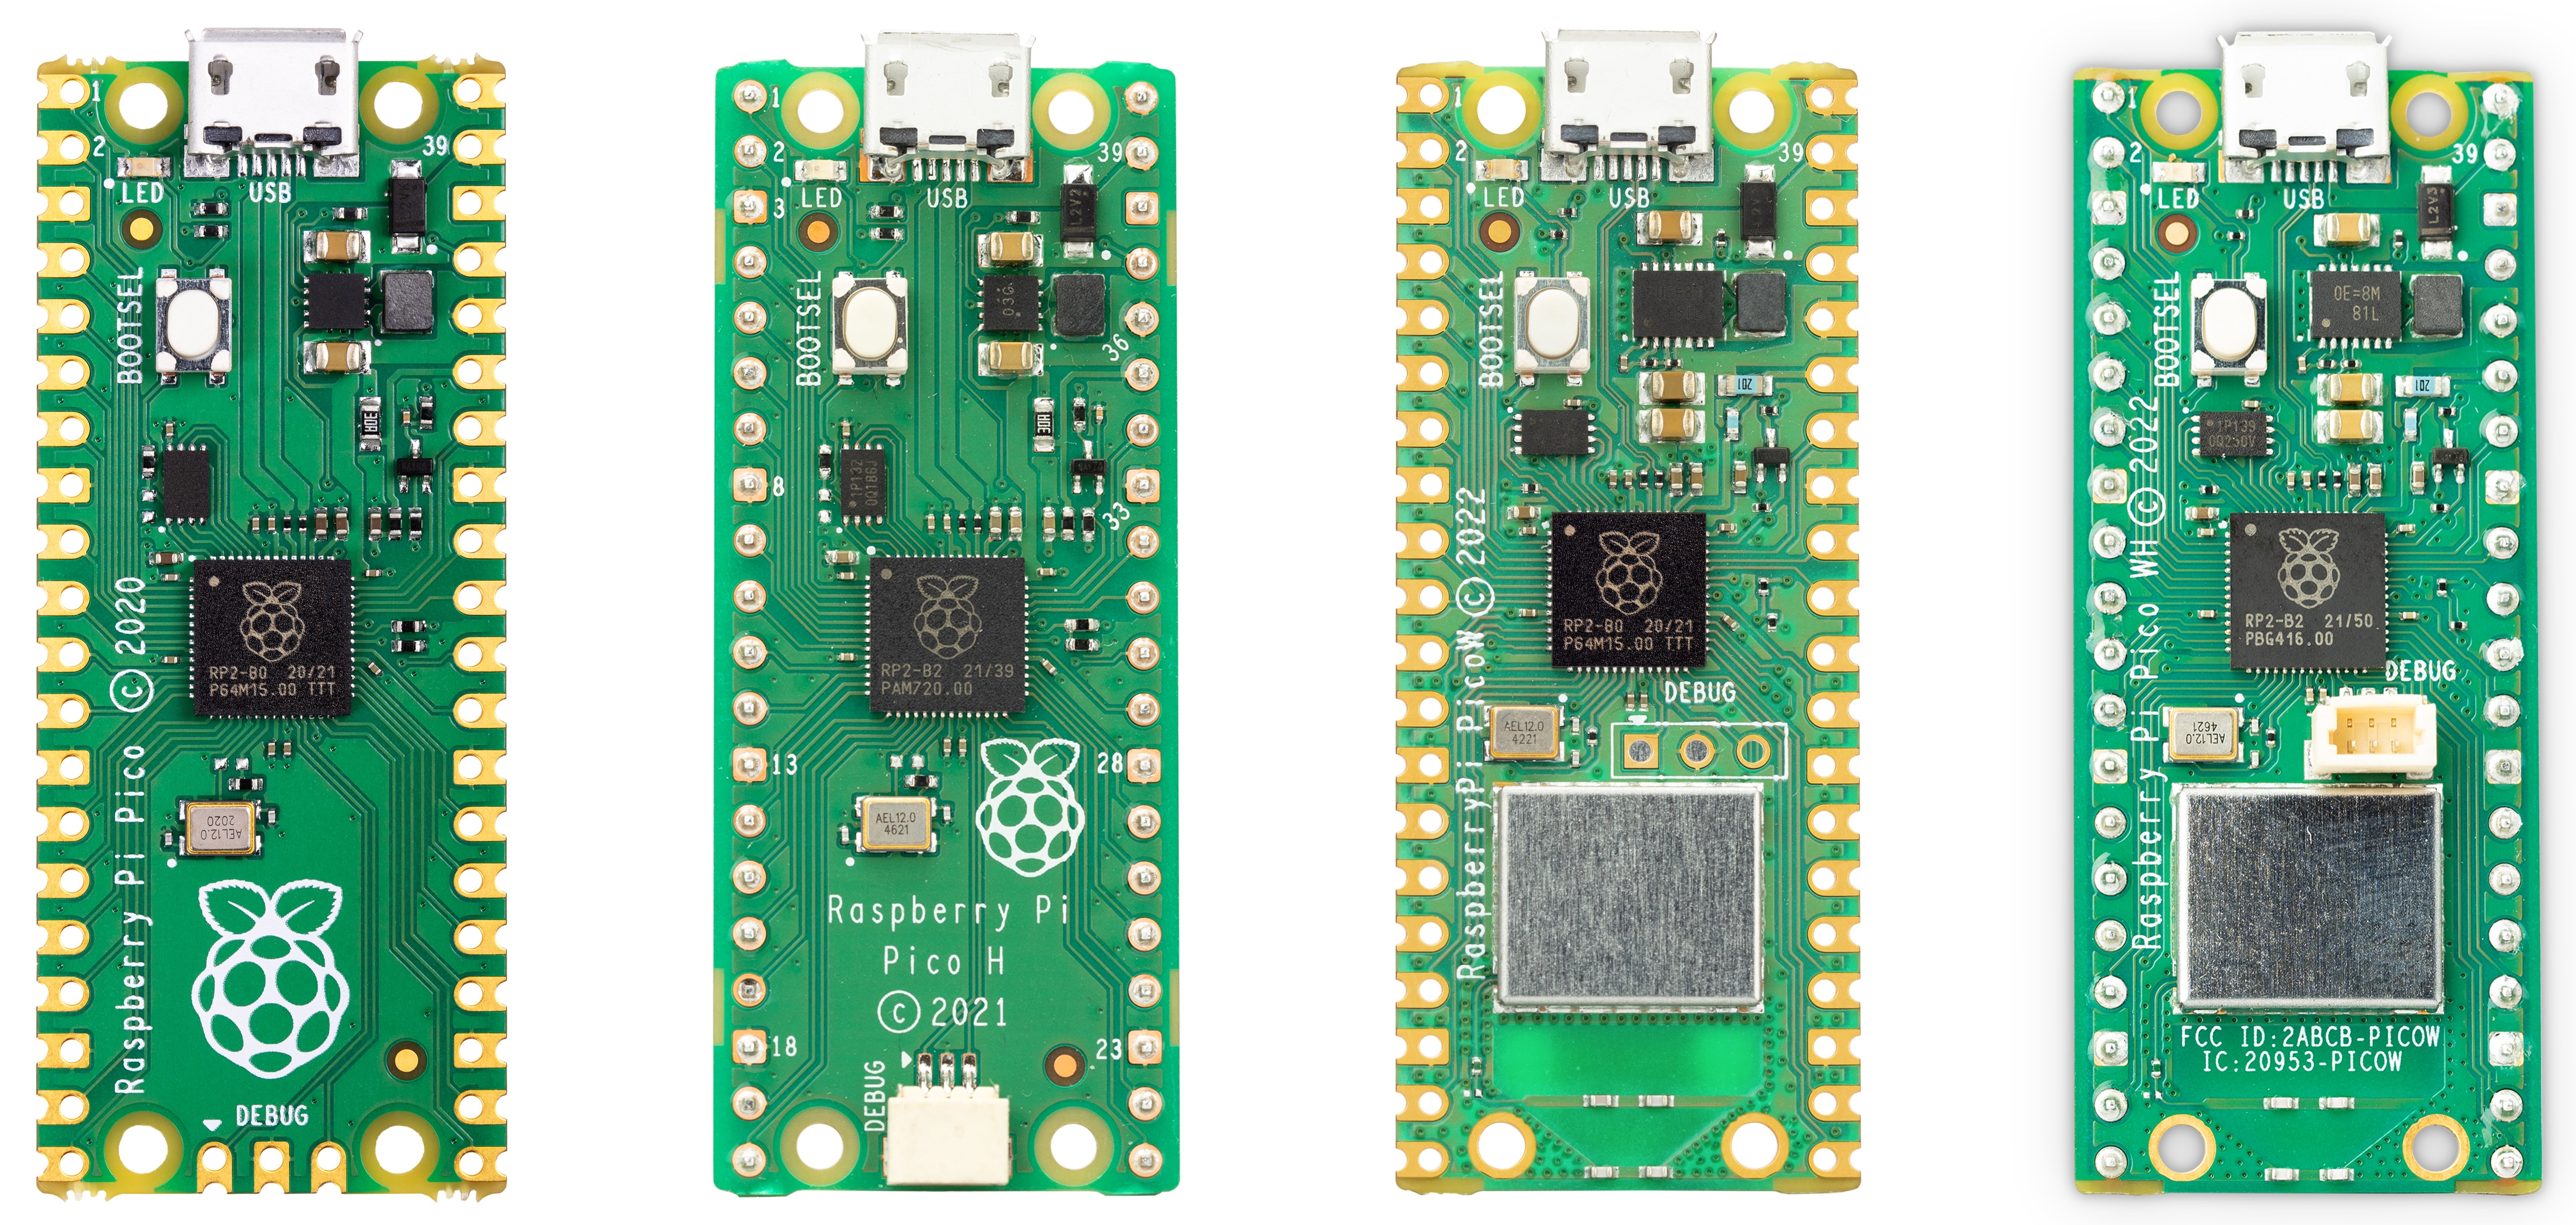
\includegraphics[width=6in]{images/pico_family.jpg}
		\caption{Raspberry Pi Pico W microcontroller board}
	\label{fig:SystemOverview}
\end{figure}
This is an image of the Raspberry Pi Pico W microcontroller board.
% This diagram shows the major external interfaces that provide the capabilities of \ThisSys.
% As are shown, the \ThisSys can provide \TBD.


% The general concept of operations (\CONOP) for this system is \TBD.








\section{Document Overview}
\label{loc:DocumentOverview}
% \DIDINFO{ALL-1.3 :: This paragraph shall summarize the purpose and contents of this
document and shall describe any security or privacy considerations associated with its use.}

This section provides information about this document's security/privacy considerations, contents, structure, and version information.

\subsection{Security and Privacy Considerations}
\label{loc:DocOverview_CUI}

%include CUI info if CUI is defined
\ifthenelse{\equal{\KNEADcuiStatus}{}}
{
	This document is not subject to \CUI restrictions.
}%endif not CUI
{% it is CUI so print CUI file info
	This document has been identified as "Controlled Unclassified Information" (\CUI).
Please follow the control block on the title page for ownership, creation, category, dissemination, and Point of Contact (\POC) information.
This information should be delineated, per \url{https://www.dodcui.mil} as:
\begin{description}[itemindent=5pt,topsep=0pt,itemsep=0pt,partopsep=0pt, parsep=0pt]
	\item[Owner] the name of the DoD Component (not required if identified in the letterhead)
	\item[Creator] identification of the office creating the document
	\item[Category] identification of the categories contained in the document
	\item[Dissemination]applicable distribution statement or limited dissemination control (LDC)
	\item[\POC]name and phone number or email of POC
\end{description}

}


This document format is based upon the guidance in the \STD{} \DID~\cite{ref__STD_DID} and the \STR{} \DID~\cite{ref__STR_DID}.
The test planning is documented following the guidelines of ISO-12207~\cite{ref__ISO_12207} and MIL-STD-498~\cite{ref__MIL_STD_498} (from which ISO-12207 originated).
This document follows the listed \STS sub-section order.
\begin{description}
	\item[Section 1] provides an overview of the system and this document.
	\item[Section 2] lists general and application-specific reference documents as well as glossary terms and acronyms. 
	\item[Section 3] summarizes the test preparations.
	\item[Section 4] provides the detailed descriptions of the tests to be performed\footnote{This section follows the \DID but places the test procedure details as the last section for each test case.}. 
	\item[Section 5] provides any applicable requirement traceability.
	\item[Section 6] if needed, lists any general notes as may be applicable.
	\item[Appendices] if needed, provide additional information as may be needed.
\end{description}


This document also is structured to serve as the basis for the system test report (\STR).
Each test is supplied with spaces for capturing pertinent hardware, software, and other log information.
Each test is divided into one or more test cases, each with detailed steps, expected results for each step, and a set of easy to read pass/fail markers for each test step.
All tests steps also provide space to fill in the results and to write notes and comments about each test step.
The goal of this style is to generate this \STR by scanning in the resultant \STS with comments using this as the  \STR Appendix-A.
In this manner, a ``written'' record of the testing is generated, thus saving money by not requiring a completely separate recording document for the \STR.

\vspace{12pt}
\DIDINFO{If this text is visible, the first instance of each section may display a summary of data item description (DID) information shown in this font.
These are displayed in small capital font and are not part of the formal document.}


\subsection{Document Version Information}
\label{loc:DocOverview_LaTeXAndSvnVersionInformation}

This document was produced in \LaTeXx and \Biberx.
The editing and document preparation were performed using MiK\TeX{} version 2.9  with the build option $[$\LaTeX{}  $\Rightarrow$ PS $\Rightarrow$ PDF$]$.
The \LaTeXx {\em svn-multi} package was used to glean SVN tracking information, when files are stored in an ``SVN'' version control system.
The style {\tt \KNEADdocumentClsName}
%, which was based on the style provided in~\cite{ref__thesisguide}, 
was used to provide the \LaTeXx and \Biberx formatting details.

% This revision of this document has the following properties:
% \begin{table}[htbp]
	% \caption{Subversion (SVN) Data}
	% \label{tab:SVNdata}
	\centering
		\begin{tabular}{|p{1.5in}|p{4.9in}|}
		%%%%%S\multicolumn{2}{c}{\bfseries SVN Information} \\
		\hline
			{\bfseries Tracking Item}  &  {\bfseries Data} \\
		\hline		
		\hline
			Repository         & \url{\svnmainurl}  \\
		\hline
			Author         & \svnauthor  \\			
		\hline
			Revision       & \svnrev     \\	
		\hline
			Rev Date       & \svndate    \\	
		\hline	
			Print Date     & \today{} \currenttime    \\	
		\hline
			\KNEADdocumentClsName\break Version     & \KNEADdocumentClsVersion    \\	
		\hline	
			\KNEADdocumentClsName\break Date        & \KNEADdocumentClsDate   \\	
		\hline
		%%%\DocumentTexName\break Version     & \DocumentTexVersion    \\	
		%%%\hline	
		%%%\DocumentTexName\break Date        & \DocumentTexDate   \\	
		\hline						
    \end{tabular}
\end{table}

